%% ----------------------------------------------------------------------------
% BIWI SA/MA thesis template
%
% Created 09/29/2006 by Andreas Ess
% Extended 13/02/2009 by Jan Lesniak - jlesniak@vision.ee.ethz.ch
%% ----------------------------------------------------------------------------
\newpage
\chapter{Approach and Implementation}
\label{ch:approach_implementation}
The main goal of this paper is to investigate a self-supervised technique on autonomous driving videos using CNN's, with an self-supervised ordering task exploiting spatiotemporal signals. In the rest of this thesis we use a similar basic approach as in previous works on using temporal coherence~\cite{misra2016,lee2017}, but then applied to videos captured by cars. As a novel line of research the usage of lidar data is explored with the aim of learning richer representations. Different versions of the task are investigated as explained in more detail in the Chapter \ref{ch:experimentsandresults}, but the basic idea of the task is as follows:
\begin{enumerate}    
\item A sequence of images is selected with sufficient motion
\item The sequence is split into separate samples with different feature maps and fed individually through one or more siamese backbone networks merged at different depths with the goal of learning generic image features.
\item The output features of all images in the sequence are subsequently used as input to an ordering network.
\item The ordering network predicts either if the ordering is correct (easy)\cite{misra2016} or the actual permutation (harder)\cite{lee2017}.
\end{enumerate}
A general implementation of this approach for the permutation order network has been provided in Figure \ref{fig:sorting_sequence}.

\section{Generating train and test data}
\begin{figure}[t]
\centering
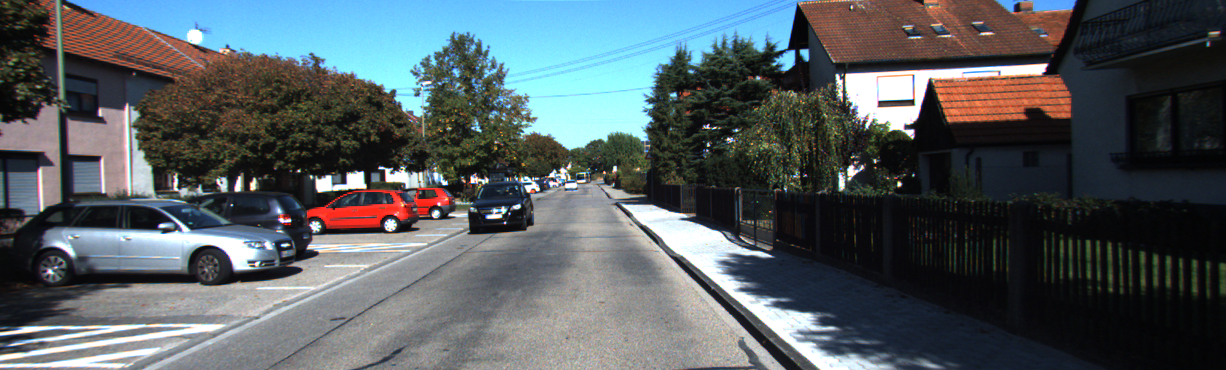
\includegraphics[width=\textwidth]{images/img_first.png}
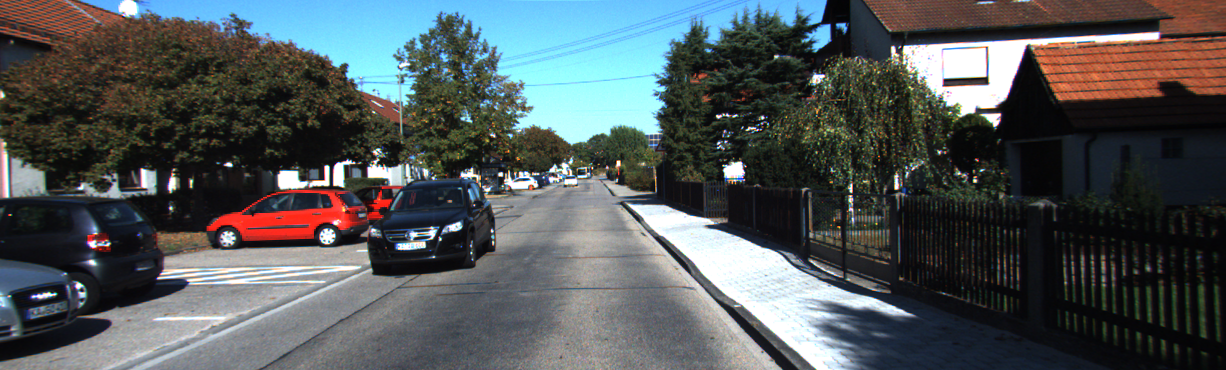
\includegraphics[width=\textwidth]{images/img_second.png}
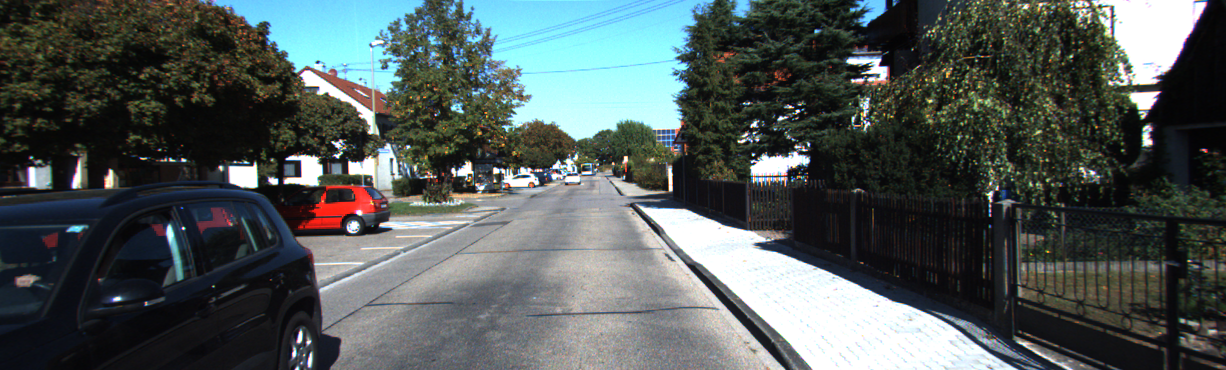
\includegraphics[width=\textwidth]{images/img_third.png}
\caption{Example of a sequence with three frames from the Kitti dataset~\cite{geiger2012}}
\label{fig:frames}
\end{figure}

As the task is unsupervised there is no need for labeled data, only a large number of video samples with precise lidar measurement. For this task one suitable choice is the Kitti\cite{geiger2012} visual odometry dataset, which is used in all experiments as it contains a large number of samples. This dataset contains a total of 22 sequences covering a total length of 39.2 km of outdoor streets divided in over 41k frames sampled at 10 Hz. It contains high-quality images from two grayscale and two color PointGrey Flea2 video cameras with 1392×512 pixel resolutions and corresponding lidar range scans from a Velodyne HDL-64E 3D laser scanner.

\begin{figure}
\centering
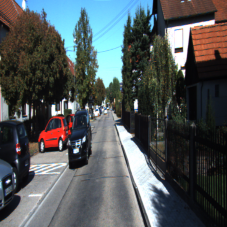
\includegraphics[width=0.49\textwidth]{images/color.png}
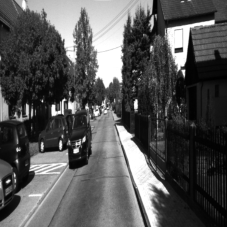
\includegraphics[width=0.49\textwidth]{images/gray.png}
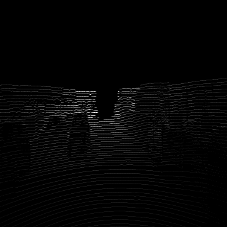
\includegraphics[width=0.49\textwidth]{images/lidar_depth.png}
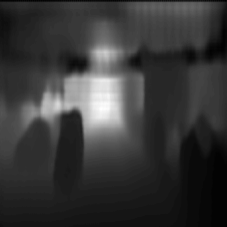
\includegraphics[width=0.49\textwidth]{images/lidar_depth_int.png}
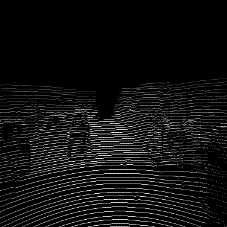
\includegraphics[width=0.49\textwidth]{images/lidar_height.png}
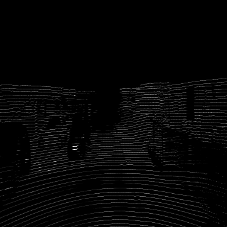
\includegraphics[width=0.49\textwidth]{images/lidar_refl.png}
\caption{Different representations of available data for the second frame displayed in Figure \ref{fig:frames} downscaled to the 227x227 version fed to the network before jittering is applied, with from top-left to bottom-right: color, grayscale, lidar depth, interpolated lidar depth, lidar height and lidar reflectance}
\label{fig:features}
\end{figure}

The dataset was split into 15 sequences for generating the training data and 7 independent sequences for testing. For generating the image data the RGB camera 02 was selected, the data from the other camera's was not used. Because the input images are of large dimensions for common backbone networks the images were first downscaled with anti-aliasing to a size of 227x227 as used in Caffenet~\cite{jia2014}. This resizing does not preserve scaling, but this is not a primary issue as all images are downsized in the same way and the structure of the objects remain clear in those smaller images. Finally for all experiments with single channel camera images, channel splitting is employed by randomly selecting one of the three RGB channels, it has been shown that this makes the data more rigid against learning low-level features then direct conversion to grayscale~\cite{lee2017}. The final images are saved as grayscale images and therefore these channel split images are simply referred as grayscale in the rest of this thesis. In other experiments with color the data is used with all RGB channels.

Properly preparing training data with sufficiently balanced difficulty is of primary importance for proper learning. Static sequences that are almost impossible to order should be prevented, but the network should also avoid learning low-level cues without semantic understanding. To generate the training and test data, sets of either 3 or 4 images both with mostly uniform and non-uniform spacing within a certain timeframe, are randomly sampled from the corresponding sequences (sequences are not all of same length, and sequences with more images are sampled more often). Then the magnitude of optical flow is calculated between the frames and only sequences with high magnitude are selected\cite{misra2016}, or more specifically where the mean intensity of the 10 highest optical flow regions is higher than a manually tuned value. An example of a selected frame is shown in Figure \ref{fig:frames}.

%[It has also been suggested to mine smaller patches from the data\cite{lee2017}.]

The 3D lidar range data is expensive to use directly as has been noted earlier, thus instead 2D views of the data are generated. Following the idea of HHA projections both a depth map and a height above ground map are produced and projected to the location of camera 02, which was used to generate the image data (the angle projection is not used in this work). Note that the height above ground is relatively easy to calculate in the case studied here, as the location of the lidar is exactly known with respect to the ground, and therefore the absolute height of all points can be directly calculated (taken the location of the wheels as ground and neglecting the possible steepness of the road. As the lidar data is sparse also an interpolated version of the depth map is produced [following an upsampling procedure from Premebida et al.\cite{premebida2014} presented earlier, to compare with the unprocessed lidar depth. Finally the reflectances are also extracted for comparison with data collected from normal images. After the features are computed the lidar data is reduced to 227x227 similar to the image data. Examples of all the investigated feature maps, both from the camera and from the lidar, are given in Figure \ref{fig:features}.

To generate a proper distribution of positive and negative samples, every image sequence is used twice for the binary ordering task with one positive (sorted) and negative (unsorted) sample added to both the training and test set. For the binary task both increasingly sorted and inversely sorted are counted as a positive (sorted) sample following Misra et al.\cite{misra2016}, who are reasoning that for certain training instances it is hard to distinguish forward and backward sorting (for example picking up a coffee or placing it down), however for the permutation task all permutations are treated separately as we actually expect this to be often identifiable in autonomous driving datasets as the cars are almost always moving in the forward direction (as in Figure \ref{fig:frames} where the forward movement can easily be identified). For the network estimating permutations, four different randomly selected permutations used for every sampled sequence. As 10,000 sequences are sampled for the training set this results in respectively 20,000 training samples and 40,000 training samples for the two variations. Similary 10,000 and 20,000 image samples have been generated for the respective test sets. 

\section{Implementation in the Caffe framework}
A convolutional neural network approach was adopted for training the task, it being the primary choice for these kind of problems in the computer vision field in the last decade. We use the widely-used Caffe framework~\cite{jia2014} to implement the different networks. The Caffe framework contains a large set of standard layers, like convolution, max-pooling, rectified linear unit (ReLu), batch normalization as well as several more infrequent ones, and contains all the logic to pass the blobs of data between those layers. The framework allows for writing custom layers in Python to access all the blobs and outputs produced by the network.

Caffe uses configuration files based on Google Protocol buffers to define networks. To facilitate the different experiments in Chapter \ref{ch:experimentsandresults} a generator was written to produce different types of networks, combining one or multiple instances (for both image and lidar data) of a variety of backbones, with a processing network. To read in images a fetcher API running in a separate process was improved from an earlier implementation by Misra et al.~\cite{misra2016}. Running in a separate process allows for preloading the images, to reduce the time spent in the data loading layer. Initially the preprocessing to down-scaled network as explained in the previous section was executed on-the-fly during loading, but it was discovered that this significantly impacted the training time and that even a separate loading thread could not keep up with this, therefore it was chosen to pregenerate the images in the correct form.

A customized input layer was implemented in Caffe, capable of loading a sequence of images of customizable length and with a selectable batch size, to faciliate the special requirements for the inspected ordering task. This layers produces the preprocessed images, with optional channel splitting and resizing. After loading the preprocessed images the same layer is used to add random jittering to every pixel, to help preventing the network from over-fitting on the data. The layer also has the possibilities to generate saliency maps, a interesting visualization method proposed by Simonyan et al.~\cite{simonyan2013}. It computes the magnitude of the first derivative of the output with respect to all the pixels in the image to find the pixels which have to be changed the least to maximally affect the class score. They show that these pixels correspond to the location of the object in object detection, as can be inspected. It can also be reasoned that these saliency maps should give an indication what object on the image the network primarily used to learn. After the initial input layer, scaling and concatenation layers are used to properly feed the images into the siamese network and bring the samples to the appropriate input of the processing network later on.

To further investigate the contents of the network, a variety of other visualization techniques have been implemented. A basic visualization layer was implemented to show the sequences with their output including probability, which was mostly used for debugging purposes. Furthermore, a simple visualizer of the weights of the various convolutional layers has been realized. Because a convolutional filter reacts strong on a shape which is similar to its own, it is to be expected that the first layer should contain a variety of edge and corner detectors. The later layers in a network are harder to interpret and visualize, but noisy patterns can be an indication for networks which have not been trained long enough or significant overfitting due to a low regularization strength\needref. Another interesting approach is visualizing the strength of the activations, which are more difficult to interpret but should generally lead to sparser and more local maps in later layers. Finally a procedure by Girshick et al.~\cite{girshick2014} was followed for visualizing the regions in the image that show maximal activation in different layers, which is primarily interesting to find the important part of the images in the deeper convolutional layers.

All the code built for this thesis can be found online on \needref.  More details about the implementation will be presented in Appendix \ref{app:implementation_details}
